% Created 2016-11-11 Fr 13:59
\documentclass[a4paper]{scrartcl}
\usepackage[utf8]{inputenc}
\usepackage[T1]{fontenc}
\usepackage{fixltx2e}
\usepackage{graphicx}
\usepackage{longtable}
\usepackage{float}
\usepackage{wrapfig}
\usepackage{rotating}
\usepackage[normalem]{ulem}
\usepackage{amsmath}
\usepackage{textcomp}
\usepackage{marvosym}
\usepackage{wasysym}
\usepackage{amssymb}
\usepackage{hyperref}
\tolerance=1000
\usepackage{siunitx}%
\usepackage{fontspec}%
\sisetup{load-configurations = abbrevations}%
\newcommand{\estimates}{\overset{\scriptscriptstyle\wedge}{=}}%
\usepackage{mathtools}%
\DeclarePairedDelimiter\abs{\lvert}{\rvert}%
\DeclarePairedDelimiter\norm{\lVert}{\rVert}%
\DeclareMathOperator{\Exists}{\exists}%
\DeclareMathOperator{\Forall}{\forall}%
\def\colvec#1{\left(\vcenter{\halign{\hfil$##$\hfil\cr \colvecA#1;;}}\right)}
\def\colvecA#1;{\if;#1;\else #1\cr \expandafter \colvecA \fi}
\usepackage{minted}
\usepackage{makecell}
\usemintedstyle{perldoc}
\usepackage{tikz}
\usetikzlibrary{arrows,automata}
\usepackage{tikz-qtree}
\usepackage{enumitem}
\setlistdepth{20}
\renewlist{itemize}{itemize}{20}
\setlist[itemize]{label=$\cdot$}
\author{Robin Heinemann}
\date{\today}
\title{Einführung in die Anwendungsorientierte Informatik (Köthe)}
\hypersetup{
  pdfkeywords={},
  pdfsubject={},
  pdfcreator={Emacs 25.1.1 (Org mode 8.2.10)}}
\begin{document}

\maketitle
\tableofcontents


\section{Klausur 10.02.2016}
\label{sec-1}

\section{Was ist Informatik?}
\label{sec-2}
"Kunst" Aufgaben mit Computerprogrammen zu lösen.
\subsection{Teilgebiete}
\label{sec-2-1}
\subsubsection{theoretische Informatik (\textbf{ITH})}
\label{sec-2-1-1}
\begin{itemize}
\item Berechenbarkeit: Welche Probleme kann man mit Informatik lösen und welche prinzipiell nicht?
\item Komplexität: Welche Probleme kann man effizient lösen?
\item Korrektheit: Wie beweist man, dass das Ergebnis richtig ist? \\
      Echtzeit: Dass das richtige Ergebnis rechtzeitig vorliegt.
\item verteilte Systeme: Wie sichert man, dass verteilte Systeme korrekt kommunizieren?
\end{itemize}
\subsubsection{technische Informatik (\textbf{ITE})}
\label{sec-2-1-2}
\begin{itemize}
\item Auf welcher Hardware kann man Programme ausführen, wie baut man dies Hardware?
\item CPU, GPU, RAM, HD, Display, Printer, Networks
\end{itemize}
\subsubsection{praktische Informatik}
\label{sec-2-1-3}
\begin{itemize}
\item Wie entwickelt man Software?
\item Programmiersprachen und Compiler: Wie kommuniziert der Programmierer mit der Hardware?\hfill \textbf{IPI}, \textbf{IPK}
\item Algorithmen und Datenstrukturen: Wie baut man komplexe Programme aus einfachen Grundbausteinen?\hfill \textbf{IAL}
\item Softwaretechnik: Wie organisiert man sehr große Projekte?\hfill \textbf{ISW}
\item Kernanwendung der Informatik: Betriebsysteme, Netzwerke, Parallelisierung\hfill \textbf{IBN}
\begin{itemize}
\item Datenbanksysteme\hfill \textbf{IDB1}
\item Graphik, Graphische Benutzerschnittstellen\hfill \textbf{ICG1}
\item Bild- und Datenanalyse
\item maschinelles Lernen
\item künstliche Intelligenz
\end{itemize}
\end{itemize}
\subsubsection{angewante Informatik}
\label{sec-2-1-4}
\begin{itemize}
\item Wie löst man Probleme aus einem anderem Gebiet mit Programmen?
\item Informationstechnik
\begin{itemize}
\item Buchhandlung, e-commerce, Logistik
\end{itemize}
\item Web programming
\item scientific computing für Physik, Biologie
\item Medizininformatik
\begin{itemize}
\item bildgebende Verfahren
\item digitale Patientenakte
\end{itemize}
\item computer linguistik
\begin{itemize}
\item Sprachverstehen, automatische Übersetzung
\end{itemize}
\item Unterhaltung: Spiele, special effect im Film
\end{itemize}
\section{Wie unterscheidet sich Informatik von anderen Disziplinen?}
\label{sec-3}
\subsection{Mathematik}
\label{sec-3-1}
Am Beispiel der Definition $a \leq b: \exists c \geq 0: a + c = b$ \\
   Informatik: \\
   Lösungsverfahren: $a - b \leq 0$, das kann man leicht ausrechen, wenn man subtrahieren und mit $0$ vergleichen kann. \\
   Quadratwurzel: $y = \sqrt{x} \Leftrightarrow y \geq 0 \wedge y^2 = x (\Rightarrow x > 0)$ \\
   Informatik: Algorithmus aus der Antike: $y = \frac{x}{y}$
iteratives Verfahren: \\
   Initial Guess $y^{(0)} = 1$
schrittweise Verbesserung $y^{(t+1)} = \frac{y^{(t)} + \frac{x}{y^{(t)}}}{2}$
\section{Informatik}
\label{sec-4}
Lösugswege, genauer Algorithmen
\subsection{Algorithmus}
\label{sec-4-1}
\textbf{schematische} Vorgehensweise mit der jedes Problem einer bestimmten \textbf{Klasse} mit \textbf{endliche} vielen \textbf{elementaren} Schritten / Operationen gelöst werden kann
\begin{itemize}
\item schematisch: man kann den Algorithmus ausführen, ohne ihn zu verstehen ($\Rightarrow$ Computer)
\item alle Probleme einer Klasse: zum Beispiel: die Wurzel aus jeder beliebigen nicht-negativen Zahl, und nicht nur $\sqrt{11}$
\item endliche viele Schritte: man kommt nach endlicher Zeit zur Lösung
\item elementare Schrite / Operationen: führen die Lösung auf Operationen oder Teilprobleme zurück, die wir schon gelöst haben
\end{itemize}
\subsection{Daten}
\label{sec-4-2}
Daten sind Symbole,
\begin{itemize}
\item die Entitäten und Eigenschaften der realen Welt im Computer representieren.
\item die interne Zwischenergebnisse eines Algorithmus aufbewahren
\end{itemize}
$\Rightarrow$ Algorithmen transformieren nach bestimmten Regeln die Eingangsdaten (gegebene Symbole) in Ausgangsdaten (Symbole für das Ergebniss).
Die Bedeutung / Interpretation der Symbole ist dem Algorithmus egal $\estimates$ "schematisch"
\subsubsection{Beispiele für Symbole}
\label{sec-4-2-1}
\begin{itemize}
\item Zahlen
\item Buchstaben
\item Icons
\item Verkehrszeichen
\end{itemize}
aber: heutige Computer verstehen nur Binärzahlen $\Rightarrow$ alles andere muss man übersetzen
Eingansdaten: "Ereignisse":
\begin{itemize}
\item Symbol von Festplatte lesen oder per Netzwerk empfangen
\item Benutzerinteraktion (Taste, Maus, \ldots{})
\item Sensor übermittelt Meßergebnis, Stoppuhr läuft ab
\end{itemize}
Ausgangsdaten: "Aktionen":
\begin{itemize}
\item Symbole auf Festplatte schreiben, per Netzwerk senden
\item Benutzeranzeige (Display, Drucker, Ton)
\item Stoppuhr starten
\item Roboteraktion ausführen (zum Beispiel Bremsassistent)
\end{itemize}
Interne Daten:
\begin{itemize}
\item Symbole im Hauptspeicher oder auf Festplatte
\item Stoppuhr starten / Timeout
\end{itemize}
\subsection{Einfachster Computer}
\label{sec-4-3}
endliche Automaten (endliche Zustandsautomaten)
\begin{itemize}
\item befinden sich zu jedem Zeitpunkt in einem bestimmten Zustand aus einer vordefinierten endlichen Zustandsmenge
\item äußere Ereignisse können Zustandsänderungen bewirken und Aktionen auslösen
\end{itemize}
\subsubsection{{\bfseries\sffamily TODO} Graphische Darstellung}
\label{sec-4-3-1}
graphische Darstellung: Zustände = Kreise, Zustandsübergänge: Pfeile
\subsubsection{{\bfseries\sffamily TODO} Darstellung durch Übergangstabellen}
\label{sec-4-3-2}
Zeilen: Zustände, Spalten: Ereignisse, Felder: Aktion und Folgezustände
\begin{center}
\begin{tabular}{llll}
Zustände $\backslash$ Ereignisse & Knopf drücken & Timeout & Timeout(Variante)\\
\hline
aus & $\Rightarrow$\{halb\} \\ \{4 LEDs an\} & \% & ($\Rightarrow$\{aus\},\{nichts\})\\
halb & ($\Rightarrow$\{voll\},\{8 LEDs an\}) & \% & ($\Rightarrow$\{aus\},\{nichts\})\\
voll & ($\Rightarrow$\{blinken an\},\{Timer starten\}) & \% & ($\Rightarrow$\{aus\},\{nichts\})\\
blinken an & ($\Rightarrow$\{aus\},\{Alle LEDs aus, Timer stoppen\}) & ($\Rightarrow$\{blinken aus\},\{alle LEDs aus, Timer starten\}) & ($\Rightarrow$\{blinken aus\},\{8 LEDs aus\})\\
blinken aus & ($\Rightarrow$\{aus\},\{Alle LEDs aus, Timer stoppen\}) & ($\Rightarrow$\{blinken an\},\{alle LEDs an, Timer starten\}) & ($\Rightarrow$\{blinken an\},\{8 LEDs an\})\\
\end{tabular}
\end{center}

Variante: Timer läuft immer (Signal alle 0.3s) $\Rightarrow$ Timout ignorieren im Zustand "aus", "halb", "voll"
\subsubsection{Beispiel 2:}
\label{sec-4-3-3}
\begin{align}
&1~0~1~1~0~1~0 &= 2 + 8 + 16 + 74 &= 90_{\text{dez}} \\
+&0~1~1~1~0~0~1 &= 1 + 8 + 16 + 32 &= 57_{\text{dez}} \\
\hline
1~&0~0~1~0~0~1~1 &= 1 + 2 + 16 + 128 &= 147_{\text{dez}}\checkmark
\end{align}
\paragraph{Implementation mit Endlichen Automaten}
\label{sec-4-3-3-1}
Prinzipen:
\begin{itemize}
\item wir lesen die Eingangsdaten von rechts nach links
\item Beide Zahlen gleich lang (sonst mit 0en auffüllen)
\item Ergebnis wird von rechts nach link ausgegeben
\end{itemize}
\paragraph{{\bfseries\sffamily TODO} Skizze der Automaten}
\label{sec-4-3-3-2}
\begin{center}
\begin{tabular}{lll}
Zustand & Ereignis & Ausgeben\\
\hline
start & (0,1) & "1"\\
start & (1,0) & "1"\\
start & (0,0) & "0"\\
start & (1,1) & "0"\\
carry = 1 & (1,1) & "1"\\
carry = 1 & (0,1) & "0"\\
carry = 1 & (1.0) & "0"\\
carry = 1 & $\emptyset$ & "1"\\
\end{tabular}
\end{center}
\textbf{Wichtig:} In jedem Zustand muss für \textbf{alle möglichen} Ereignisse eine Aktion und Folgezustand definiert werden.
Vergisst man ein Ereignis zeigt der Automat undefiniertes Verhalten, also einen "Bug".
Falls keine sinvolle Reaktion möglich ist: neuer Zustand: "Fehler" $\Rightarrow$ Übergang nach "Fehler",
Aktion: Ausgeben einer Fehlermeldung
\subparagraph{{\bfseries\sffamily TODO} Skizze Fehlermeldung}
\label{sec-4-3-3-2-1}
Ein endlicher Automat hat nur ein Speicherelement, das den aktuelen Zustand angibt. Folge:
\begin{itemize}
\item Automat kann sich nicht merken, wie er in den aktuellen Zustand gekommen ist ("kein Gedächnis")
\item Automat kann nicht beliebig weit zählen, sondern nur bis zu einer vorgegebenen Grenze
\end{itemize}
\begin{center}
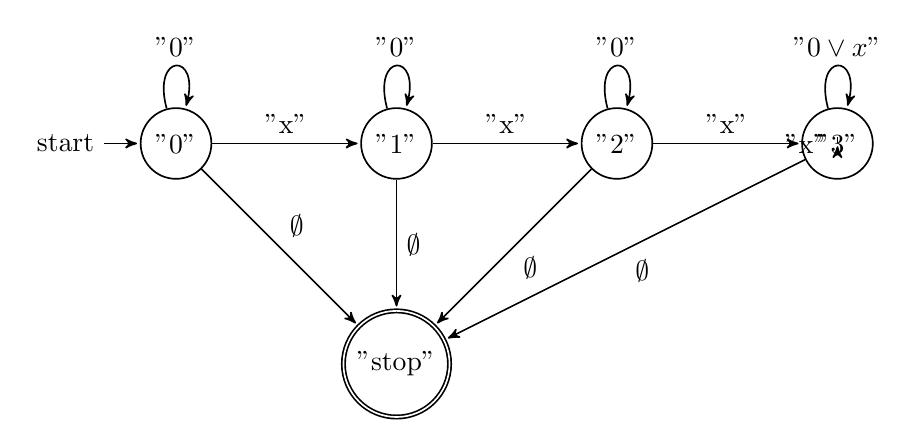
\begin{tikzpicture}[->,>=stealth',shorten >=1pt,auto,node distance=2.8cm, semithick]
\node[initial,state] (0) {"0"};
\node[state] (1) [right of=0] {"1"};
\node[state] (2) [right of=1]{"2"};
\node[state] (3) [right of=2]{"3"};
\node[accepting,state] [below of=1] (end) {"stop"};
\path (0) edge [loop above] node {"0"} (0)
(0) edge node {"x"} (1)
(0) edge node {$\emptyset$} (end)
(1) edge [loop above] node {"0"} (1)
(1) edge node {"x"} (2)
(1) edge node {$\emptyset$} (end)
(2) edge [loop above] node {"0"} (2)
(2) edge node {"x"} (3)
(2) edge node {$\emptyset$} (end)
(3) edge [loop above] node {"$0\vee x$"} (3)
(3) edge node {"x"} (3)
(3) edge node {$\emptyset$} (end);
\end{tikzpicture}
\end{center}
Insgesamt: Man kann mit endlichen Automaten nur relativ einfache Algorithmen implementieren. (nur reguläre Sprachen)
Spendiert man zusätzlichen Specher, geht mehr:
\begin{itemize}
\item Automat mit Stack-Speicher (Stapel oder Keller) $\Rightarrow$ Kellerautomat (Kontextfreie Sprachen)
\item Automat mit zwei Stacks oder äquivalent Turing-Maschine kann alles auführen, was man intuitiv für berechenbar hält
\end{itemize}
Markov Modelle: endliche Automaten mit probabilistischen Übergangen.
Bisher: Algorithmen für einen bestimmten Zweck (Problemklasse)
Frage: Gibt es einen universellen Algorithms für alle berechenbare Probleme?
Betrache formale Algorithmusbeschreibung als Teil der Eingabe des universellen Algorithmus.
\section{Substitutionsmodell (funktionale Programmierung)}
\label{sec-5}
\begin{itemize}
\item einfaches Modell für arithmetische Berechnung "Taschenrechner"
\item Eingaben und Ausgaben sind Zahlen (ganze oder reelle Zahlen). Zahlenkonstanten heißten "Literale"
\item elementare Funktionen: haben eine oder mehere Zahlen als Argumente (Parameter) und liefern eine Zahl als Ergebnis (wie Mathematik):
\begin{itemize}
\item add(1,2) $\rightarrow$ 3, mul(2,3) $\rightarrow$ 6, analog sub(), div(), mod()
\end{itemize}
\item Funktionsaufrufe können verschachtelt werden, das heißt Argumente kann Ergebnis einer anderen Funktion sein
\begin{itemize}
\item mul(add(1,2),sub(5,3)) $\rightarrow$ 6
\end{itemize}
\end{itemize}
\subsection{Substitutionsmodell}
\label{sec-5-1}
Man kann einen Funktionsaufruf, dessen Argument bekannt ist (das heißt Zahlen sind) durch den Wert des Ergebnisses ersetzen ("substituieren"). Geschachtelte Ausdrücke lassen sich so von innen nach außen auswerten.
\[mul(add(1,2),sub(5,3))\]
\[mul(3,sub(5,3))\]
\[mul(3,2)\]
\[6\]
\begin{itemize}
\item Die arithmetischen Operationene add(), sub(), mul(), div(), mod() werden normalerweise von der Hardware implementiert.
\item Die meisten Programmiersprachen bieten außerdem algebraische Funktionen wie: sqrt(), sin(), cos(), log()
\begin{itemize}
\item sind meist nicht in Hardware, aber vorgefertigte Algorithmen, werden mit Programmiersprachen geliefert, "Standardbibilothek"
\end{itemize}
\item in C++: mathematisches Modul des Standardbibilothek: "cmath"
\item Für Arithmetik gebräuchlicher ist "Infix-Notation" mit Operator-Symbolen "+", "-", "*", "/", "\%"
\item mul(add(1,2),sub(5,3)) $\Leftrightarrow$ ((1+2)*(5-3))
\begin{itemize}
\item oft besser, unter anderem weil man Klammer weglassen darf
\begin{enumerate}
\item "Punkt vor Strichrechnung" 3+4*5 $\Leftrightarrow$ 3+(4*5), mul, div, mod binden stärker als add, sub
\item Operatoren gleicher Präzedenz werden von links nach rechts ausgeführt (links-assoziativ) \\
          1+2+3-4+5 $\Leftrightarrow$ ((((1+2)+3)-4)+5)
\item äußere Klammer kann man weglassen (1+2)$\Leftrightarrow$ 1+2
\end{enumerate}
\end{itemize}
\item Computer wandeln Infix zuerst in Prefix Notation um
\begin{enumerate}
\item weggelassene Klammer wieder einfügen
\item Operatorensymbol durch Funktionsnamen ersetzen und an Prefix-Position verschieben
\[1 + 2 + 3 * 4 / (1 + 5) - 2\]
\[(((1 + 2) + ((3 * 4) / (1 + 5))) - 2)\]
\[sub(add(add(1,2),div(mul(3,4),add(1,5))), 2)\]
\[sub(add(3,div(12,6)), 2)\]
\[sub(add(3,2), 2)\]
\[sub(5, 2)\]
\[2\]
\end{enumerate}
\end{itemize}
\subsection{Bäume}
\label{sec-5-2}
\begin{itemize}
\item bestehen aus Knoten und Kanten (Kreise und Pfeile)
\item Kanten verbinden Knoten mit ihren Kind-knoten
\item jeder Koten (außer der Wurzel) hat genau ein Elternteil ("parent node")
\item Knoten ohne Kinder heißen Blätter ("leaves / leaf node")
\item Teilbaum
\begin{itemize}
\item wähle beliebigen Knoten
\item entferne temporär dessen Elternkante, dadurch wird der Knoten temporär zu einer Wurzel, dieser Knoten mit allen Nachkommen bildet wieder einen Baum (Teilbaum des Orginalbaumes)
\end{itemize}
\item trivialer Teilbaum hat nur einen Knoten
\item Tiefe: Abstand eines Knotens von der Wurzel (Anzahl der Kanten zwischen Knoten und Wurzel)
\begin{itemize}
\item Tiefe des Baums: maximale Tiefe eines Knoten
\end{itemize}
\end{itemize}
\subsubsection{Beispiel}
\label{sec-5-2-1}
\[1 + 2 + 3 * 4 / (1 + 5) - 2\]
\[sub(add(add(1,2),div(mul(3,4),add(1,5))), 2)\]
\begin{center}
\Tree [ .sub [ .add [ .add 1 2 ] [ .div [ .mul 3 4 ] [ .add 1 5 ] ] ] 2 ]
\end{center}
\subsection{Rekursion}
\label{sec-5-3}
Rekursiv $\estimates$ Algorithmus für Teilproblem von vorn.
\subsection{Prefixnotation aus dem Baum rekonstruieren}
\label{sec-5-4}
\begin{enumerate}
\item \label{algstart1} Wenn die Wurzel ein Blatt ist: Drucke die Zahl
\item sonst:
\begin{itemize}
\item Drucke Funktionsnamen
\item Drucke "("
\item Wiederhole den Algorithmus ab \ref{algstart1} für das linke Kind (Teilbaum mit Wurzel = linkes Kind)
\item Drucke ","
\item Wiederhole den Algorithmus ab \ref{algstart1} für das rechte Kind (Teilbaum mit Wurzel = rechtes Kind)
\item Drucke ")"
\end{itemize}
$\Rightarrow$ \[sub(add(add(1,2),div(mul(3,4),add(1,5))), 2)\]
\end{enumerate}
\subsection{Prefixnotation aus dem Baum rekonstruieren}
\label{sec-5-5}
\begin{enumerate}
\item \label{algstart2} Wenn die Wurzel ein Blatt ist: Drucke die Zahl
\item sonst:
\begin{itemize}
\item Drucke Funktionsnamen
\item Drucke "("
\item Wiederhole den Algorithmus ab \ref{algstart2} für das linke Kind (Teilbaum mit Wurzel = linkes Kind)
\item Drucke Operatorsymbol
\item Wiederhole den Algorithmus ab \ref{algstart2} für das rechte Kind (Teilbaum mit Wurzel = rechtes Kind)
\item Drucke ")"
\end{itemize}
$\Rightarrow$ \[sub(add(add(1,2),div(mul(3,4),add(1,5))), 2)\]
\end{enumerate}
$\Rightarrow$ \textbf{inorder}
\subsection{Berechnen des Werts mit Substitutionsmethode}
\label{sec-5-6}
\begin{enumerate}
\item \label{algstart3} Wenn Wurzel dein Blatt gib Zahl zurück
\item sonst:
\begin{itemize}
\item Wiederhole den Algorithmus ab \ref{algstart3} für das linkes Kind (Teilbaum mit Wurzel = rechtes Kind), speichere Ergebnis als "lhs"
\item Wiederhole den Algorithmus ab \ref{algstart3} für das rechte Kind (Teilbaum mit Wurzel = rechtes Kind), speichere Ergebnis als "rhs"
\item berechne funktionsname(lhs,rhs) und gebe das Ergebnis zurück
\end{itemize}
\end{enumerate}
$\Rightarrow$ \textbf{postorder}
\section{Maschienensprachen}
\label{sec-6}
\begin{itemize}
\item optimiert für die Hardware
\item Gegensatz: höhere Programmiersprachen (c++)
\begin{itemize}
\item optimiert für Programmierer
\end{itemize}
\item Compiler oder Interpreter übersetzen Hoch- in Maschinensprache
\end{itemize}
\subsection{Umwandlung in Maschinensprache}
\label{sec-6-1}
\begin{enumerate}
\item Eingaben und (Zwischen)-Ergebnisse werden in Speicherzellen abgespeichert $\Rightarrow$ jeder Knoten im Baum bekommt eine Speicherzelle
\item Speicherzellen für Eingaben initialisieren
\begin{itemize}
\item Notation: SpZ $\leftarrow$ Wert
\end{itemize}
\item Rechenoperationen in Reihenfolge des Substitutionsmodell ausführen und in der jeweiligen Speicherzelle speichern
\begin{itemize}
\item Notation: SpZ-Ergebniss $\leftarrow$ fname SpZArg1 SpZArg2
\end{itemize}
\item alles in Zahlencode umwandeln
\begin{itemize}
\item Funktionsnamen:
\begin{center}
\begin{tabular}{lr}
Opcode & Wert\\
\hline
init & 1\\
add & 2\\
sub & 3\\
mul & 4\\
div & 5\\
\end{tabular}
\end{center}
\end{itemize}
\end{enumerate}
\section{Funktionale Programmierung}
\label{sec-7}
\begin{itemize}
\item bei Maschienensprache werden Zwischenergebnisse in Speicherzellen abgelegt
\item das ist auch in der funktionalen Programmierung eine gute Idee
\item Speicherzellen werden duch Namen (vom Programmierer vergeben) unterschieden
\end{itemize}
\subsection{Beispiel}
\label{sec-7-1}
Lösen einer quadratischen Gleichung:
\[ax^2 + bx + c = 0\]
\[x^2 - 2px + q = 0, p = -\frac{b}{2a},q=\frac{c}{d}\]
\[x_2 = p + \sqrt{p^2 - q},x_2 = p - \sqrt{p^2 - q}\]
ohne Zwischenergebnisse:
\[x_1 \leftarrow add(div(div(b,a),-2),sqrt(sub(mul(div(b,a),-2),div(div(b,a)-1)),div(c,a)))\]
mit Zwischenergebniss und Infix Notation
\[p\leftarrow b / c / -2~\text{oder}~p\leftarrow -0.5 * b / a\]
\[a\leftarrow c / a\]
\[d\leftarrow sqrt(p*p - q)\]
\[x_1\leftarrow p + d\]
\[x_2\leftarrow p - d\]
\subsection{Vorteile von Zwischenergebnissen}
\label{sec-7-2}
\begin{enumerate}
\item lesbarer
\item redundante Berechnung vermieden. Beachte: In der funktionalen Programmierung können die Speicherzellen nach der Initialisierung nicht mehr verändert werden
\item Speicherzellen und Namen sind nützlich um Argumente an Funktionen zu übergeben $\Rightarrow$ Definition eigener Funktionen
\begin{minted}[]{cpp}
function sq(x) {
   return x * x
}
\end{minted}
$\Rightarrow$ $d \leftarrow sqrt(sq(p) - q)$
Speicherzelle mit Namen "x" für das Argument von $sq$
\end{enumerate}
\subsection{Funktionale Programmierung in c++}
\label{sec-7-3}
\begin{itemize}
\item in c++ hat jede Speicherzelle einen Typ (legt Größe und Bedeutung der Speicherzelle fest)
\begin{itemize}
\item wichtige Typen
\begin{center}
\begin{tabular}{ll}
int & ganze Zahlen\\
double & reelle Zahlen\\
std::string & Text\\
\end{tabular}
\end{center}
int: $12,-3$ \\
       double: $-1.02,1.2e-4 = 1.2*10^{-4}$ \\
       std::string: "text"
\end{itemize}
\item Initialisierung wird geschrieben als "typename spzname = Wert;"
\begin{minted}[]{cpp}
double a = ...;
double b = ...;
double c = ...;
double p = -0.5 b / a;
double q = c / a;
double d = std::sqrt(p*p - q);
double x1 = p + d;
double x2 = p - d;
std::cout << "x1: " << x1 << ", x2: " << x2 << std::endl;
\end{minted}
\item eigene Funktionen in C++
\begin{minted}[]{cpp}
// Kommentar (auch /* */)
type_ergebnis fname(type_arg1 name1, ...) {
	// Signatur / Funkitonskopf / Deklaration
	return ergebnis;                      
	/* Funktionskörper / Definition / Implementation */
}
\end{minted}
\begin{itemize}
\item ganze Zahl quadrieren:
\begin{minted}[]{cpp}
int sq(int x) {
	return x*x;
}
\end{minted}
\item reelle Zahl quadrieren:
\begin{minted}[]{cpp}
double sq(double x) {
	return x*x;
}
\end{minted}
\item beide Varianten dürfen in c++ gleichzeitig definiert sein $\Rightarrow$ "function overloading" $\Rightarrow$ c++ wählt automatisch die richtig Variable anhand des Argumenttypes ("overload resolution")
\begin{minted}[]{cpp}
int x = 2;
double y = 1.1
int x2 = sq(x) // int Variante
double y2 = sq(y) // double Variante
\end{minted}
\item jedes c++-Programm muss genau eine Funktion names "main" haben. Dort beginnt die Programmausführung.
\begin{minted}[]{cpp}
int main() {
	Code;
	return 0;
}
\end{minted}
\begin{itemize}
\item return aus der "main" Funktion ist optional
\end{itemize}
\item Regel von c++ für erlaubte Name
\begin{itemize}
\item erstes Zeichen: Klein- oder Großbuchstaben des englischen Alphabets, oder "\_"
\item optional: weitere Zeichen oder, "\_" oder Ziffer 0-9
\end{itemize}
\item vordefinierte Funktionen:
\begin{itemize}
\item eingebaute $\estimates$ immer vorhanden
\begin{itemize}
\item Infix-Operatoren $+,-,*,/,\%$
\item Prefix-Operatoren $operator+,operator-,\ldots$
\end{itemize}
\item Funktion der Standardbibilothek $\estimates$ müssen "angefordert" werden
\begin{itemize}
\item Namen beginnen mit "std::", "std::sin,\ldots{}"
\item sind in Module geordnet, zum Beispiel
\begin{itemize}
\item cmath $\Rightarrow$ algebraische Funktion
\item complex $\Rightarrow$ komplexe Zahlen
\item string $\Rightarrow$ Zeichenkettenverarbeitung
\end{itemize}
\item um ein Modul zu benutzen muss man zuerst (am Anfang des Programms) sein Inhaltsverzeichnis importieren (Header includieren) $\rightarrow$ \#include <name>
\begin{minted}[]{cpp}
#include <iostream>
#include <string>
int main() {
	std::cout << "Hello, world!" << std::endl;
	std::string out = "mein erstes Programm\n";
	std::cout << out;
	return 0;
}
\end{minted}
\end{itemize}
\end{itemize}
\item overloading der arithmetischen Operationene
\begin{itemize}
\item overloading genau wie bei $sq$
\begin{itemize}
\item 3 * 4 $\Rightarrow$ int Variante
\item 3.0 * 4.0 $\Rightarrow$ double Variante
\item 3 * 4.0 $\Rightarrow$ automatische Umwandliung in höheren Typ, hier "double" $\Rightarrow$ wird als 3.0 * 4.0 ausgeführt
\end{itemize}
\end{itemize}
\item $\Rightarrow$ Devision unterscheidet sich
\begin{itemize}
\item Integer-Division: 12 / 5 = 2 (wird abgerundet)
\item Double-Division: 12.0 / 5.0 = 2.4
\item -12 / 5 = 2 ($\Rightarrow$ truncated Division)
\item 12.0 / 5.0 = 2.4
\item Gegensatz (zum Beispiel in Python)
\begin{itemize}
\item floor division $\Rightarrow$ wird immer abgerundet $\Rightarrow$ -12 / 4 = -2
\end{itemize}
\end{itemize}
\end{itemize}
\end{itemize}
% Emacs 25.1.1 (Org mode 8.2.10)
\end{document}